\chapter{Analýza a návrh řešení}

\section{Představa aplikace}
\label{chapter:requirements}

Navržená ontologie hudby by pro naše účely hudebního přehrávače měla popisovat hudbu takovým způsobem, aby pokryla požadavky a očekávání uživatele hudebního přehrávače.


Potenciální posluchač, než začne samotnou hudbu poslouchat, potřebuje napřed požadovanou hudbu nalézt (ať již na svém kapesním přehrávači či ve webové aplikaci).
Nejjednodušší cesta k nalezení konkrétní hudby samozřejmě nastává v situaci, kdy uživatel přesně ví, jaký název písně či interpreta požaduje. Uživatel si ale pouze s tímto základním vyhledáváním nevystačí.
Uživatel může mít např. chuť poslouchat jeho oblíbený žánr a nezáleží mu na konkrétním interpretovi. 

Nebo naopak. V běžném životě si člověk zcela přirozeně řekne, že se mu líbí určitý hudební interpret, a že by rád poslouchal jemu podobnou hudbu. Proto stejně tak přirozené by mělo být tuto myšlenku převést do hudebního přehrávače.
Převeďme si tuto myšlenku do věty v přirozeném jazyce, tedy např. "Líbí se mi hudba Michaela Jacksona". 
Pokud vám někdo tuto větu řekne a zároveň vás požádá, abyste mu sdělili podobnou hudbu, jste schopni mu odpovědět, a to na základě znalostí, které máte či které si dohledáte.
 
Stejnou komunikaci mezi lidmi se tedy pokusíme převést do počítačové podoby. 
Dotázaný člověk v našem příkladu, jak již bylo řečeno, odpovídal na základě \textit{znalostí}. Bez potřebných znalostí by totiž nemohl tazateli odpovědět.
Pro úspěšné převedení takové komunikace tedy evidentně musíme počítači zajistit potřebné znalosti, aby i on věděl stejně jako vědí lidé, že Michaelu Jacksonovi je podobná např. Whitney Houston s Madonnou, zatímco např. takový Marilyn Manson s ním nemá nic společného. 

Ideálním nástrojem pro počítač, aby mohl odvozovat takovéto vzájemné vztahy, je zcela jistě ontologie.
Pomocí ontologie totiž můžeme vyrobit potřebnou znalostní bázi, z které pak náš program bude čerpat a na jejím základě může vyhodnocovat potřebné znalosti a ve výsledku tak nabízet pro uživatele relevantní informace.

Další možností, kterou se tato práce dále nezabývá, vyhledávání příbuzné hudby je cestou přes porovnávání zvukového signálu.

Uživatel může mít dále touhu poslouchat směsici různých žánrů. Má chuť např. na britský pop říznutý Rock\&Rollem.
Nebo je uživatel dokonce milovník a znalec konkrétních hudebních nástrojů či by si jen rád poslechl nějakou kvalitní elektrickou kytaru.

Všechny výše zmíněné požadavky se v práci pokusíme uspokojit formou webové aplikace.

\section{Současná řešení}

    Podívejme se nyní na současný stav souvisejících řešení.
    
    Se základním relačním databázovým modelem pro popis hudby přišly projekty \textit{FreeDB} \cite{freedb} a \textit{MusicBrainz} \cite{musicbrainz}.
    Tyto dvě služby nabízejí velkou databázi hudebních interpretů, jejich děl apod. Dále zmiňme např. projekt DBpedia, který se úspěšně snaží transformovat data z Wikipedie do strukturovanější, sémantičtější podoby \cite{dbpedia}. 
    
    V r. 2004 vznikla služba MusicBrainz Metadata Vocabulary \cite{musicbrainzmetadatavoc}, která využila databázi MusicBrainz a vytvořila z ní ontologii. Tehdy ještě ale MusicBrainz nebyl vyvinut natolik jako dnes.
    Novější a známější projekt \textit{Music Ontology}, který vymyslel Frédérick Giasson, opět čerpá z MusicBrainz databáze a vytváří novou hudební ontologii využívající W3C RDF technologii \cite{mo}. 
    Music Ontology tedy ve výsledku umožňuje SPARQL dotazování nad MusicBrainz databází, a to právě díky RDF, ve kterém je ontologie napsána (resp. samotná ontologie je vyjádřená pomocí RDF/XML).
    
    Navíc Music Ontology využívá dalších praktických ontologií, jako je \textit{The Friend of a Friend (FOAF) project}, který umožňuje sdílení a propojení informací o lidech, místech a dalších věcech, které jsou dostupné na webu \cite{foaf}.
    Music Ontology dále používá \textit{Event Ontology}, kterou používá k popisu různých událostí (např. koncerty a vystoupení, nahrávky) \cite{event} současně s \textit{Timeline Ontology} popisující informace z hlediska času \cite{timeline}.

    Praktickým vyústěním Music Ontology jsou např. aplikace Pandora\footnote{Pandora \url{http://www.pandora.com/}}, velmi populární služba last.fm\footnote{last.fm \url{http://www.last.fm/}} a zřejmě nejčerstvější BBC Music\footnote{BBC Music \url{http://www.bbc.co.uk/music}}.

\section{Návrh hudební ontologie}

Naší snahou je vymodelovat vlastní hudební ontologii za vhodného použití FOAF příp. Event/Timeline ontologie.

Ontologii budeme vyvíjet v editoru Protégé 4.0 a výsledek budeme ukládat do formátu RDF/XML, jelikož je tento druh serializace nejběžněji používaný. RDF/XML formát používá mimo jiné právě i již zmíněná Music Ontology a jazyk OWL 2 jej vyžaduje jako primární syntaxi (což je videt např. z obr. \ref{img:owl2}).

Volně se necháme inspirovat projektem Music Ontology, nicméně se pokusíme hudební ontologii postavit sami dle svého nejlepšího uvážení. 
Výslednou ontologii pak můžeme s Music Ontology porovnat.

Při vytvoření ontologie v Protégé tedy naimportujeme FOAF a Event ontologii (předpokládáme jejich využití) a začínáme modelovat vlastní hudební ontologii.

Zvykem je začínat od třídy \textit{Thing}, tedy "věc", která zastřešuje všechny další třídy. Lépe se nám pak uvažuje hierarchie, lépe si ji dovedeme představit - pokud by tato třída neexistovala, všechny její podtřídy by chaoticky "létaly" ve vzduchu. Její existence nám pomáhá ke klasické stromové struktuře, na kterou jsme navyklí (viz obr. \ref{img:thing2}). Stejný obrázek dále ukazuje, které třídy jsme v naší ontologii nějakým způsobem použili (samozřejmě některé mají další podtřídy, na obrázku nezobrazené).

\begin{figure}[h]
\begin{center}
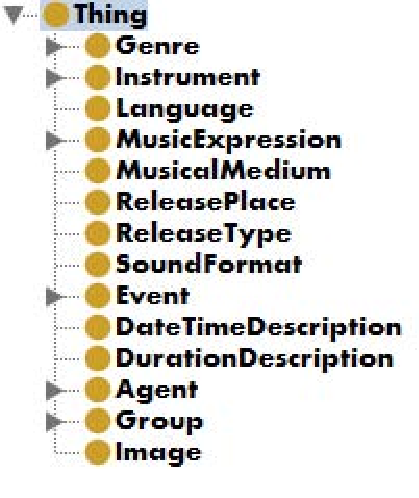
\includegraphics[width=5cm]{figures/thing2}
\caption{Nadtřída Thing obsahující všechny použité třídy}
\label{img:thing2}
\end{center}
\end{figure}

Třídy a podtřídy jsou mezi sebou definované vztahem "IS-A", tedy každá potřída rozšiřuje vlastnosti svého rodiče. Vztah mezi třídy znázorňuje obrázek \ref{img:thing}

\begin{figure}[h]
\begin{center}
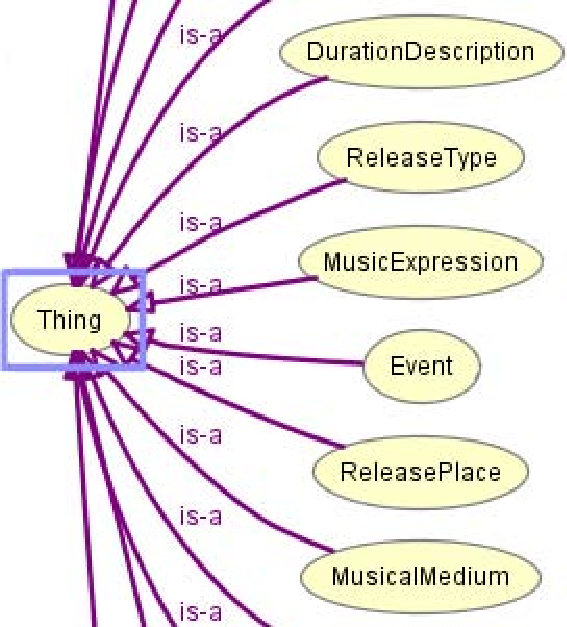
\includegraphics[width=6.5cm]{figures/thing}
\caption{Ukázka "IS-A" vztahu mezi třídou-podtřídou}
\label{img:thing}
\end{center}
\end{figure}

Hierarchii tříd jsme modelovali podle našeho uvážení tak, aby vyhovovala našemu účelu. 

Ontologii Event jsme použili na třídu Event, ve které jsou podtřídy definující konkrétní typ události (viz obr. \ref{img:event}).

\begin{figure}[h]
\begin{center}
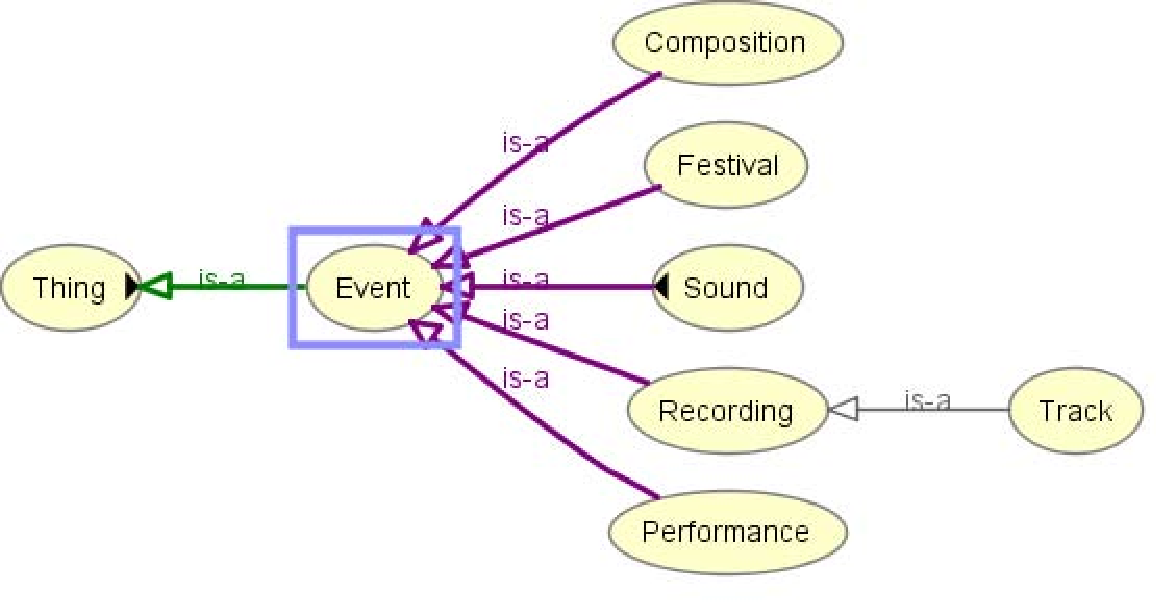
\includegraphics[width=13cm]{figures/event}
\caption{Třída Event patřící do importované Event Ontology a její rozšíření v rámci naší ontologie}
\label{img:event}
\end{center}
\end{figure}

Třídy Agent, Person, Group a další jsou definované přes importovanou ontologii FOAF (viz obr.\ref{img:foafclasses}).
V návrhu ontologie jsme využili i vztahy definované FOAF ontologií. Např. jména instancím či přiřazení člena do určité kapely jsme přidávali přes FOAF vlastnosti foaf:name či foaf:member.

Význam FOAF a Event vztahů a tříd je dán definicí podle těchto ontologií a tím je zajištěna jejich srozumitelnost např. při sdílení ontologie na webu. 

\begin{figure}[h]
\begin{center}
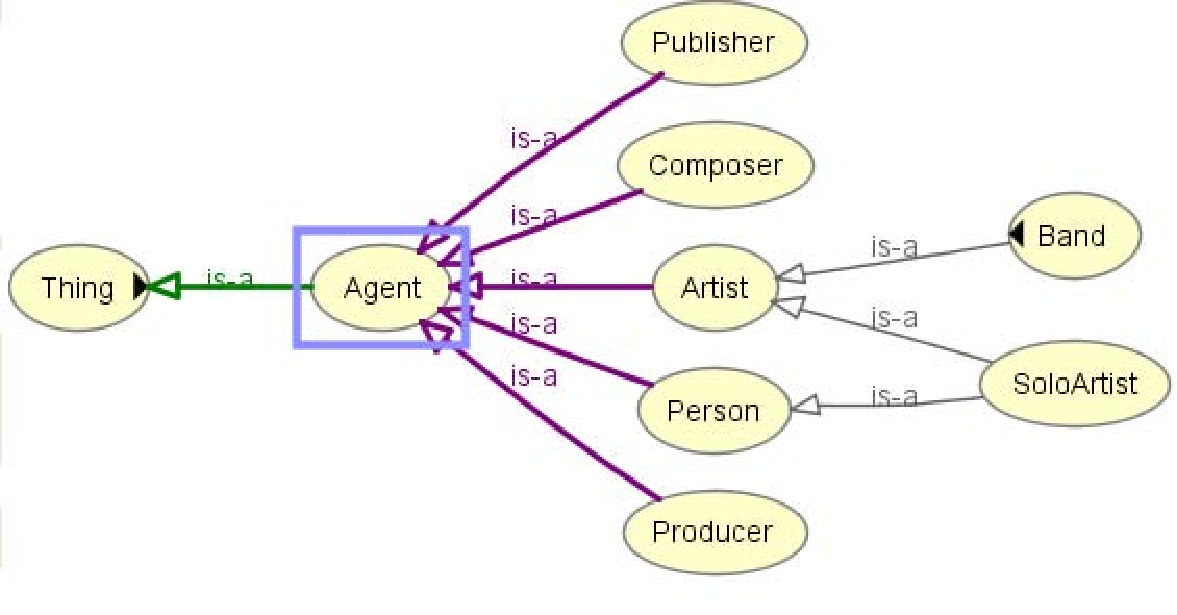
\includegraphics[width=13cm]{figures/foafclasses}
\caption{Ukázka třídy Agent a jejích podtříd. Agent a Person jsou definovány z FOAF ontologie a tím je zajištěn jejich patřičný význam.}
\label{img:foafclasses}
\end{center}
\end{figure}

Výsledná struktura tříd navržené ontologie je zobrazena na obrázku \ref{img:ontoFinal}. 
Z úsporných důvodu jsou však hudební nástroje a žánry zobrazeny zvlášť. 

Pro hudební nástroje jsem vytvořil hiearchii tříd podle celosvětově uznávané hudební klasifikace Hornbostel-Sachs \cite{hornsachs}.
Tím naší ontologii vdechneme potenciál pro možné využití mezi hudebně odbornou veřejností. Částečné (z úsporných důvodů) schéma hudebních nástrojů je vyobrazeno na obrázku \ref{img:ontoFinalInstruments}. Celá struktura hudebních nástrojů je dostupná na stránkách projektu.

Struktura hudebních žánrů byla vytvořena více či méně podle \cite{allmusic} a výsledek naleznete na obr. \ref{img:ontoFinalGenres}.

\textbf{Pozn.}: Všechny schémata použité v této části kapitoly zobrazující strukturu tříd jsou zobrazením pouze tříd, nikoliv instancí.

Plnou dokumentaci hudební ontologie vytvořenou přes OWLDoc plugin\footnote{OWLDoc plugin do Protégé \url{http://www.co-ode.org/downloads/owldoc/}} naleznete na webových stránkách projektu\footnote{Stránky projektu \url{http://martindoubravsky.cz/ctu/}}.

Výslednou hudební ontologii včetně naplněných testovacích instancí si je možné prohlížet taktéž online pomocí aplikace \textit{Ontology Browser} vytvořené projektem CO-ODE \footnote{Ontology Browser \url{http://code.google.com/p/ontology-browser/}}.

\section{Návrh webové aplikace}
\label{chapter:webappdesign}

Pro vytvořenou ontologii navrhneme webovou aplikaci, která bude umožňovat uživateli v ontologii vyhledávat podle požadavků sepsaných v kapitole \ref{chapter:requirements}.
Tyto požadavky se pokusíme sepsat v následující podkapitole funkčních požadavků.

\subsection{Funční požadavky}
\label{chaper:funcrequirements}
\begin{itemize}
\item Vyhledávání podobných interpretů.
\item Vyhledávání interpretů podle více žánrů.
\item Vyhledávání interpretů na základě hudebních nástrojů.
\item Vyhledávání podle písní a alb.
\end{itemize}

Pro webové prostředí použiji programovací jazyk PHP, a to z důvodu, že je mi tento jazyk bližší než např. Java, ve které by aplikace postavit samozřejmě šla také.
Dále volím PHP z důvodu možného budoucího srovnání jazyků PHP a Java, jak si vedou při zpracovávání ontologií (v současné době vyvíjí kolega jiný projekt postavený také na ontologii a právě na Javě, výsledky proto bude možné porovnat).

Pro práci s ontologií jsem na základě analýzy zvolil systém ARC, což je RDF systém pro sémantický web běžící na PHP.
ARC je zdarma jako open-source, je snadno použitelný a umožňuje dotazovat se přímo pomocí SPARQL dotazů.

Při vývoji webové aplikace budeme dbát na to, aby zůstala oddělena aplikační vrstva od vrstvy prezentační. 

Výstup aplikace bude formou webové stránky v jazyce HTML 5, což je nová stále se ještě vyvíjející verze jazyka HTML, přinášející podstatné změny a novinky (často kontroverzní). 

Vyhledávání v ontologii provedeme přes SPARQL výrazy vhodně zakomponované do PHP a ARC struktury.
Zřejmě přes HTML formulář vyplněný uživatelem odešleme hledaný výraz přes Hypertext Transfer Protocol (HTTP) a metodu GET. V PHP aplikační části tento hledaný výraz odbavíme a předáme systému ARC, který nad výrazem provede SPARQL dotazy a vrátí výsledek.
Výsledek uživateli zobrazíme přes jednoduché a použitelné grafické rozhraní.